% AMR Paper Figure Macros

% =============

\newcommand{\figchal}{
	\begin{figure}[t]
    \centering
  \begin{subfigure}{\columnwidth}
    \centering
    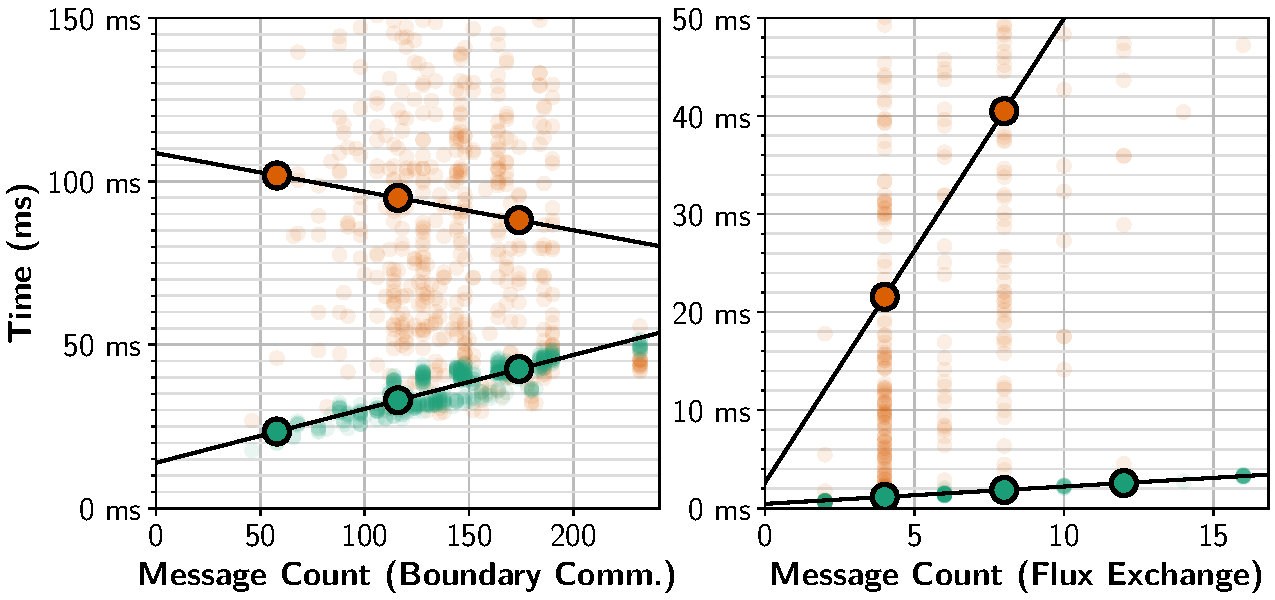
\includegraphics
    [width=\columnwidth]
    {data/figs/amr_msgcnt_regr.pdf}
    \caption{Correlation between message counts and timing}
    \label{fig:amr:chal:regr}
  \end{subfigure}
  \begin{subfigure}{0.9\columnwidth}
    \centering
    
\includegraphics
    [trim=0cm 0cm 0cm 0cm, clip, width=\columnwidth]
    {data/figs/amr_lesson_volfunc_v2_short_zoom.pdf}
    \caption{Coarse vs fine-grained telemetry from an AMR code}
    \label{fig:amr:chal:vol}
  \end{subfigure}

  \caption{Telemetry
    challenges in AMR codes.
	(Top) Initial telemetry shows poor correlation between work (message counts) and
    communication time.
    Tuning for system-level issues improves correlation and telemetry reliability.
	(Bottom) Fine-grained telemetry reveals subtle
    performance anomalies affecting average collective time by $3\times$.
  } \label{fig:amr:chal}
  \end{figure}
}

% =============

\newcommand{\figtunehw}{
  \begin{figure}[t]
    \centering
		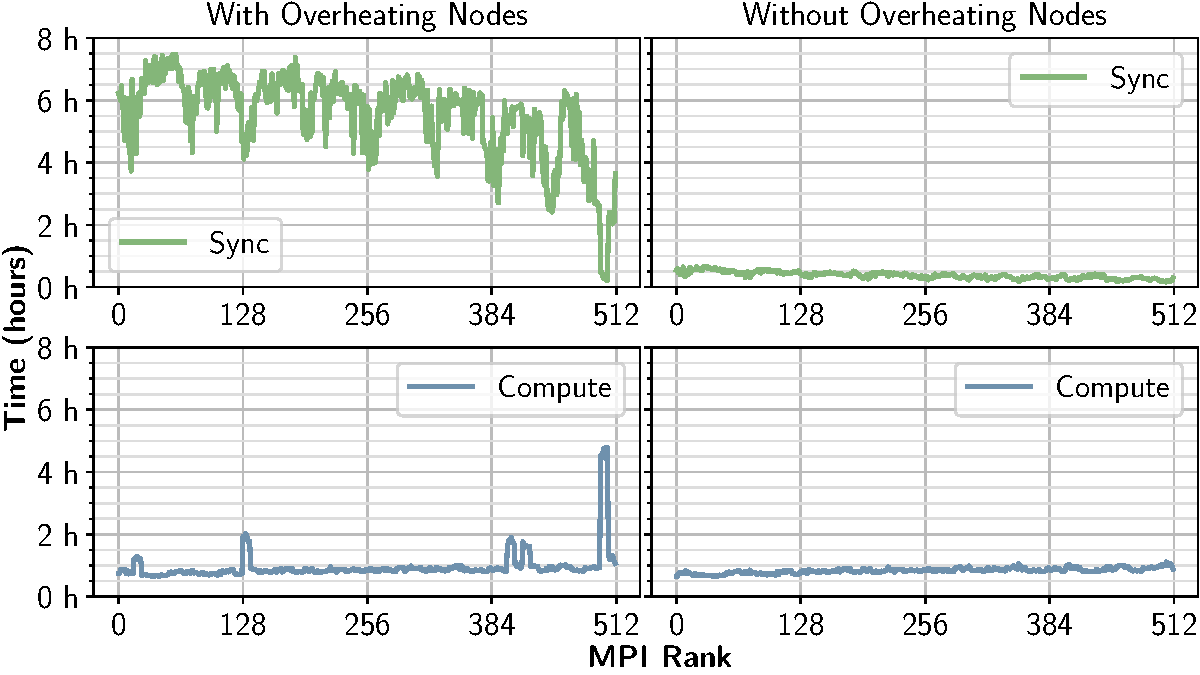
\includegraphics [width=\columnwidth]
		{data/figs/amr_lesson_throttling_v4.pdf}
		\caption{
        Profiling data from early runs affected by CPU throttling. Compute times on impacted ranks were inflated by up to 4$\times$ and appeared in clusters of 16, leading to elevated synchronization delays across the system. Pruning affected nodes reduced overall runtime by 3$\times$ by lowering synchronization overhead
    }
		\label{fig:amr:perf:throttle}
	\end{figure}
}

\newcommand{\figtunesw}{
  \begin{figure}[t]
    \centering
		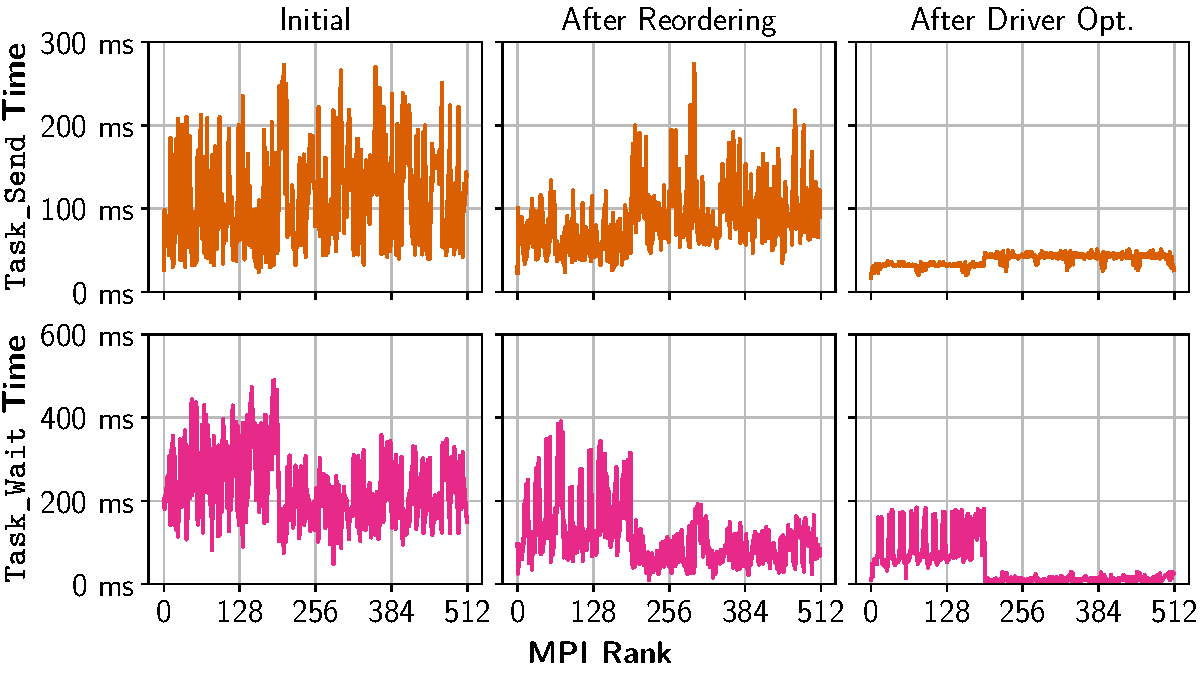
\includegraphics [width=\columnwidth]
    {data/figs/amr_lesson_ordering_v5.pdf}
		\caption{
        Rankwise boundary communication performance before and after two optimizations. Prioritizing sends in the task schedule reduced noise, revealing faint performance trends. Subsequent queue size tuning further reduced variance, clarifying the underlying telemetry structure.
        }
		\label{fig:amr:perf:order}
	\end{figure}
}

% =============

\newcommand{\figcritp}{
	\begin{figure}[t]
  \centering
  \begin{subfigure}{0.5\textwidth}
    \centering
    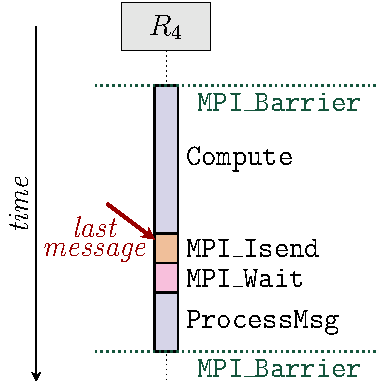
\includegraphics
    [width=0.99\linewidth, height=0.12\textheight, keepaspectratio]
    {data/figs/amr_criticalpath2.pdf}
    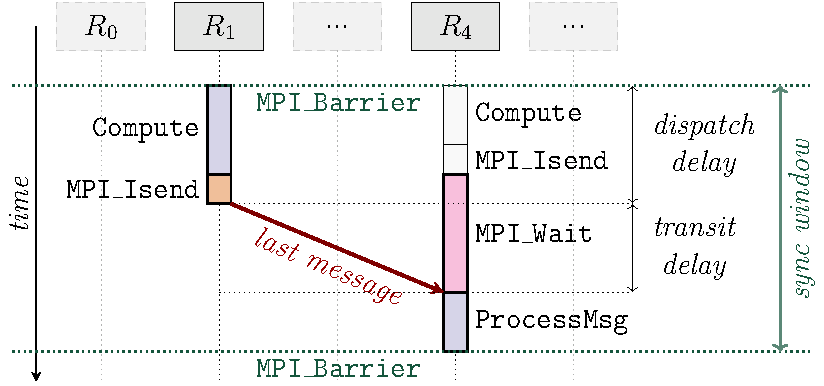
\includegraphics
    [width=0.99\linewidth, height=0.12\textheight, keepaspectratio]
    {data/figs/amr_criticalpath.pdf}
    \caption{Critical path examples in single and multi-rank scenarios}
    \label{fig:amr:model:2rcp}
  \end{subfigure}

  \vspace{10pt}

  \begin{subfigure}{0.4\textwidth}
    \centering
    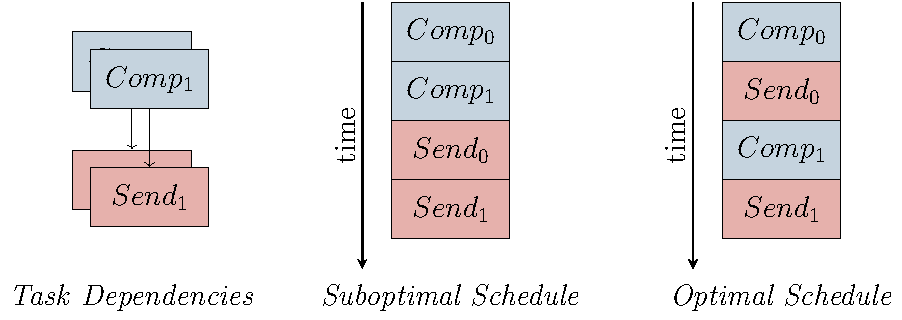
\includegraphics
    [width=0.99\linewidth]
    {data/figs/amr_sendorder_v2.pdf}
    \caption{Impact of send ordering on task scheduling}
    \label{fig:amr:model:so}
  \end{subfigure}

  \caption{Critical paths within
    a synchronization window. (Top) Single- vs two-rank critical paths,
    demonstrating how delay chains can be purely local or involve exactly two ranks
    with one P2P communication round. (Bottom) A task schedule for two blocks,
    demonstrating the impact of ordering.
    Prioritizing $Send_0$ reduces its dispatch time without affecting $Send_1$, minimizing its
    potential to create a critical path.
  } \label{fig:amr:model}
  \end{figure}
}

\newcommand{\figoctree}{
	\begin{figure}[t]
  \centering
  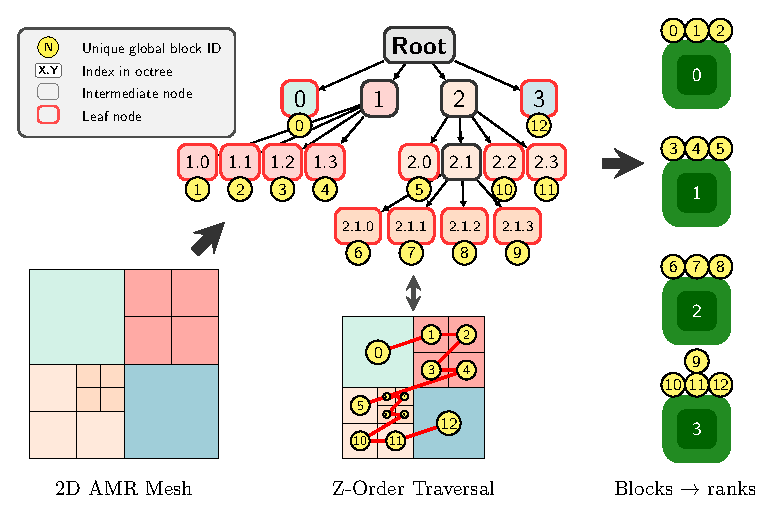
\includegraphics
  [width=\columnwidth]
  {data/figs/amr_octree.pdf}

  \caption{Example of an adaptively refined mesh, octrees, and Z-order
    Space-Filling Curves (SFCs) in two dimensions.
    Mesh blocks correspond to octree nodes with refinement creating child nodes.
    Sequential block IDs are assigned to leaf blocks using a depth-first traversal, equivalent to a
    Z-Order SFC.
    Contiguous block ID ranges are then assigned to simulation ranks to balance block counts while preserving
    locality.
  }\label{fig:amr:bg:octree}
  \end{figure}
}

% =============

\newcommand{\tableruns}{
  \begin{table}[h]
    \begin{threeparttable}
      \begin{tabular*}{\columnwidth}{@{\extracolsep{\fill}} cccccc @{}}

        \toprule
        \textbf{\textsc{ranks}}
        & \textbf{\textsc{mesh size}}
        & $\mathbf{t_{total}}$
        & $\mathbf{t_{lb}}$
        & $\mathbf{n_{initial}}$
        & $\mathbf{n_{final}}$                                         \\
        \midrule
        512  & $128^3$                     & 30,590 & 1,213 & 512   & 2,080 \\
        1024 & $128^2 \times 256$          & 43,088 & 4,576 & 1,024 & 3,824 \\
        2048 & $128 \times 256^2$          & 43,042 & 4,699 & 2,048 & 4,848 \\
        4096 & $256^3$                     & 53,459 & 9,392 & 4,096 & 8,968 \\
        \bottomrule
      \end{tabular*}

      \begin{tablenotes}[flushleft]
        \small
        \item $t_{total}$: total timesteps, $t_{lb}$: timesteps invoking load-balancing
        \item $n_{init}$: initial block count, $n_{final}$: final block count
      \end{tablenotes}
    \end{threeparttable}

    \label{tab:amr:results}\caption{ Problem configurations for Sedov Blast Wave
      3D experiments.
      All configurations use $16^3$ block size, initializing with one block per rank to ensure meaningful
      placement impact at all scales.
      The number of blocks increases through refinement as the shock wave propagates, with final block
      counts shown in the rightmost column.
    }
  \end{table}
}

% =============

\newcommand{\figevalbwwidemini}{
  \begin{figure*}
    \begin{subfigure}{\textwidth}
      \centering
			
\includegraphics[
      trim=0cm 0.2cm 0cm 0.2cm,
      clip,
      width=\textwidth]{data/figs/amr_blastwave_runtime_wide.pdf}
      \caption{Performance breakdown by execution phase and policy}
      \label{fig:amr:eval:runtime:wide}
    \end{subfigure}
    \begin{subfigure}{0.5\textwidth}
      \centering
			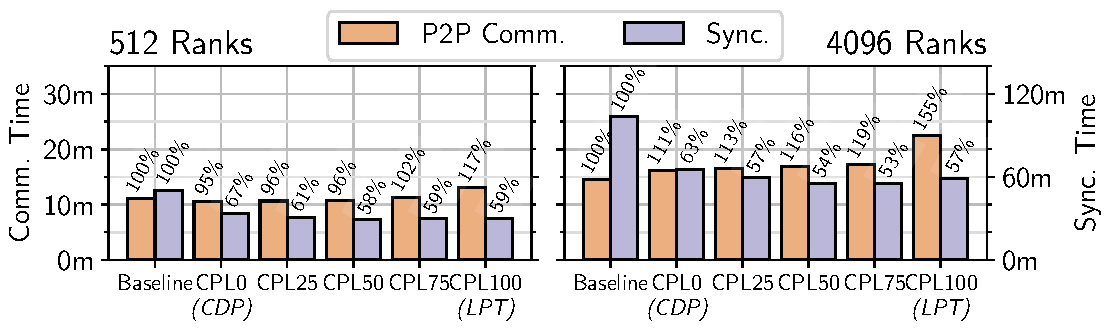
\includegraphics[
      trim=0cm 0.2cm 0cm 0.2cm,
      clip,
      width=\textwidth]{data/figs/amr_blastwave_tradeoff_wide_mini.pdf}
      \caption{Communication and synchronization time tradeoffs}
      \label{fig:amr:eval:tradeoff:wide}
    \end{subfigure}
    \begin{subfigure}{0.5\textwidth}
      \centering
			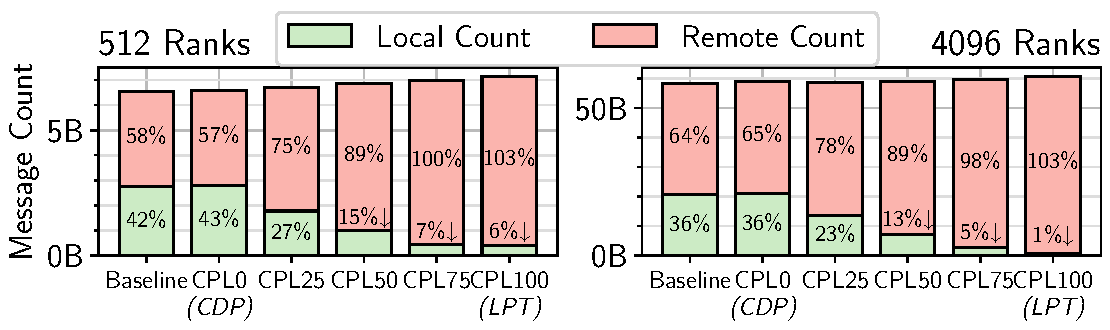
\includegraphics[
      trim=0cm 0.2cm 0cm 0.2cm,
      clip,
      width=\textwidth]{data/figs/amr_blastwave_comm_wide_mini.pdf}
      \caption{Locality analysis by message volume} \label{fig:amr:eval:comm:wide}
    \end{subfigure}

    \caption{Runtime statistics comparing
      different load-balancing policies across multiple scales (512--4096 ranks). \\
      (Top) Total runtime, classified into phases.
      CPL50 performs best, with up to 21.6\% runtime reduction over baseline.
      (Bottom, left) Clear tradeoff emerges between communication time (increasing with X) and
      synchronization time (decreasing with X), demonstrating how CPLX enables controlled balance
      between these competing factors.
      (Bottom, right) Message patterns
      show that increasing X reduces local in favor of remote communication,
      providing evidence for the locality-performance tradeoff.}
    \label{fig:amr:eval:main:wide}
  \end{figure*}
}

% =============

\newcommand{\figmicro}{
  \begin{figure}[t]
    \begin{subfigure}{0.5\textwidth}
      \centering
      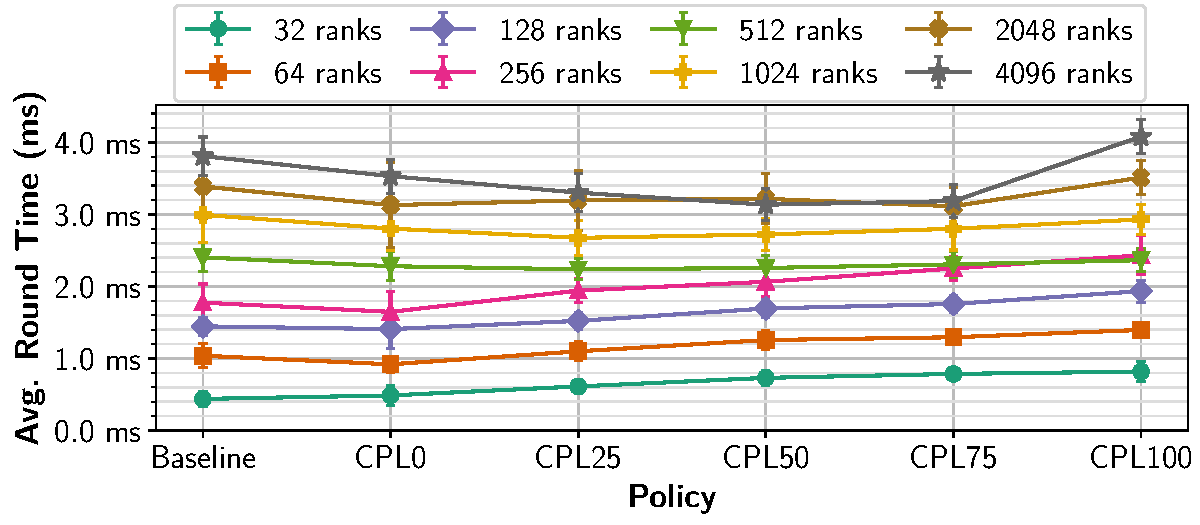
\includegraphics[width=\columnwidth]
      {data/figs/amr_meshdriver_locbench.pdf}
      \caption{Boundary communication latency vs. policies (\commbench)}
      \label{fig:amr:eval:loc}
    \end{subfigure}

    \begin{subfigure}{0.5\textwidth}
      \centering
      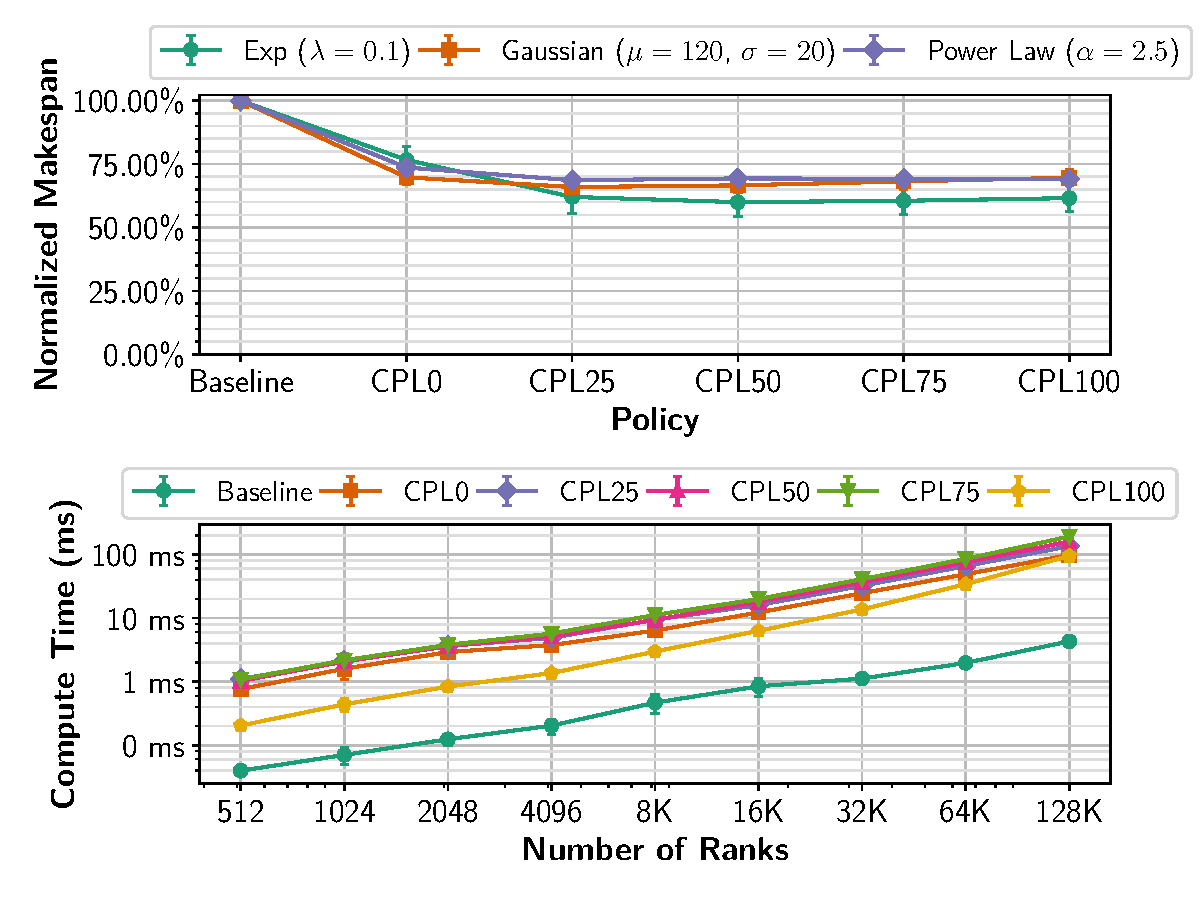
\includegraphics
      [trim=.1cm 7.6cm .1cm .1cm, clip, width=\columnwidth]
      {data/figs/amr_scaling.pdf}
      \caption{
        Load balance quality vs. polices (\scalebench)
      }
      \label{fig:amr:eval:scal_a}
    \end{subfigure}
    \begin{subfigure}{0.5\textwidth}
      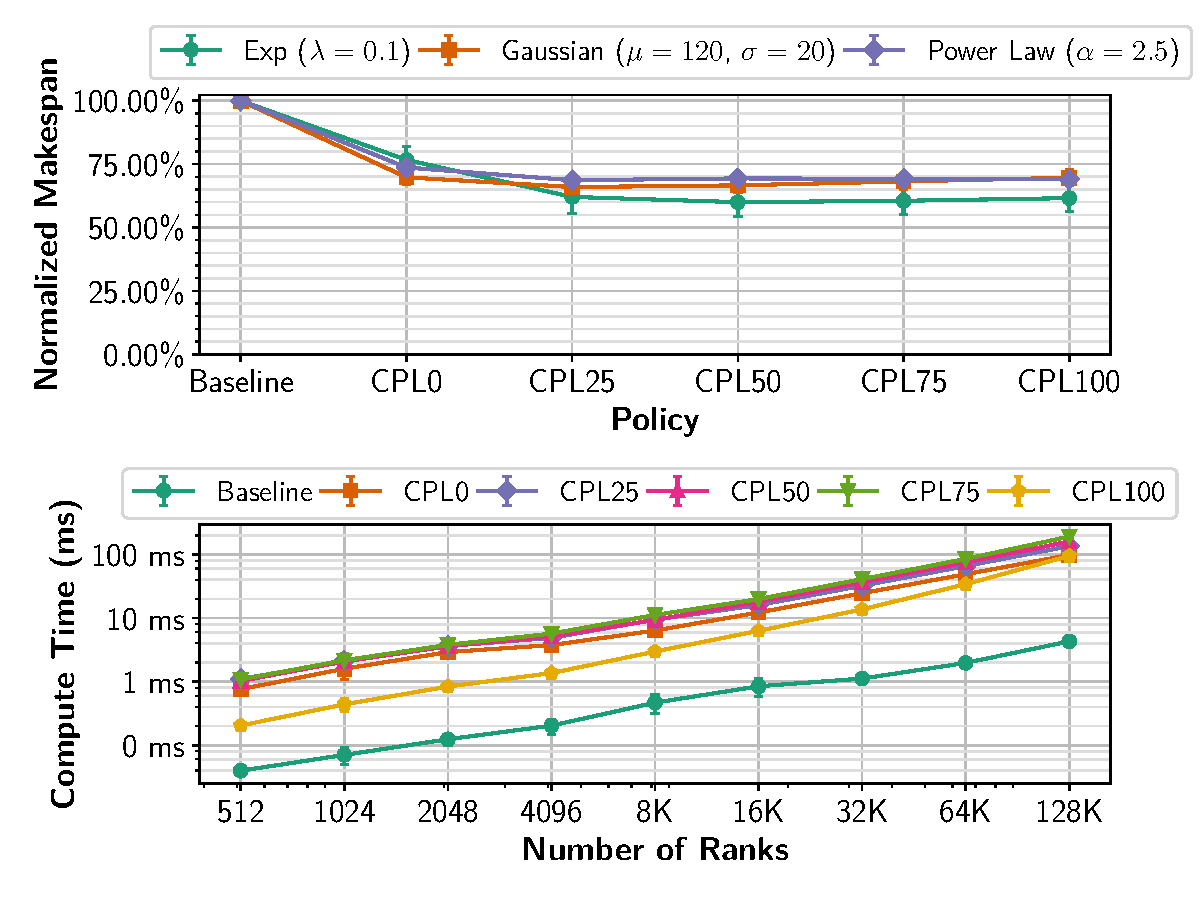
\includegraphics
      [trim=.1cm .4cm .1cm 7.6cm, clip, width=\columnwidth]
      {data/figs/amr_scaling.pdf}
      \caption{
        Policy compute cost vs. simulated rank count (\scalebench)
      }
      \label{fig:amr:eval:scal_b}
    \end{subfigure}
    \caption{
      (Top) Boundary communication round latency vs. locality at different scales, measured using \commbench.
      Locality modestly affects round latency ($\pm0.5ms$).
      At larger scales, strict locality preservation surprisingly becomes counterproductive, as it
      results in communication hotspots relative to hybrid placements.
      \\
      (Middle) Average makespans from CPLX placements with three synthetic distributions.
      While LPT performs best across all distributions, the bulk of the benefits are realized with
      $X=25$.
      \\
      (Bottom) Compute time for CPLX as a function of scale, averaged across three
      synthetic distributions.
      Compute time stays below 10ms until 16K ranks, and can be reduced beyond that scale using smaller
      parallel instances.
    } \label{fig:amr:eval:micro}
  \end{figure}
}
